\section{Building Applications on \sys}
\label{sec:app}

We built five applications on top of \sys, one that uses the basic \sys\ APIs, one that implements and uses a high-level, extended API, and two that offload data processing tasks to \MN{}s, and one that splits computation across \CN{}s and \MN{}s.

\ulinebfpara{Image compression.}
We build a simple image compression/decompression utility that runs purely at \CN.
Each client of the utility (\eg, a Facebook user) has its own collection of photos, 
stored in two arrays at \MN{}s, one for compressed and one for original, both allocated with \alloc.
Because clients' photos need to be protected from each other, we use one process
per client to run the utility.
The utility simply reads a photo from \MN\ using \Cliosysread, compresses/decompresses it,
and writes it back to the other array using \Cliosyswrite.
Note that we use compression and decompression as an example of image processing.
These operations could potentially be offloaded to \MN{}s.
However, in reality, there can be many other types of image processing that are more complex and are hard and costly to implement in hardware, necessitating software processing at \CN{}s.
We implemented this utility with 1K C code in 3 developer days.

\ulinebfpara{Radix tree.}
To demonstrate how to build a data structure on \sys\
using \sys's extended API, we built a radix tree with linked lists and pointers.
Data-structure-level systems like AIFM~\cite{AIFM} could follow this example to make simple changes in their libraries to run on \sys.
%where all nodes in a layer is linked in a list and each node points a link list
%of its children.
We first built an extended pointer-chasing functionality in FPGA at the \MN\ which follows pointers in a linked list and performs a value comparison
at each traversed list node. It returns either the node value when there is a match or null when the next pointer becomes null. 
We then expose this functionality to \CN{}s as an extended API.
The software running at \CN\ allocates a big contiguous remote memory space using \alloc\ and uses this space to store radix tree nodes. Nodes in each layer are linked to a list.
To search a radix tree, the \CN\ software goes through each layer of the tree and calls the pointer chasing API until a match is found.
We implemented the radix tree with 300 C code at \CN\ and 150 SpinalHDL code at \sysboard\ in less than one developer day.


{
\begin{figure*}[th]
\begin{minipage}{\figWidthSix}
\begin{center}
\centerline{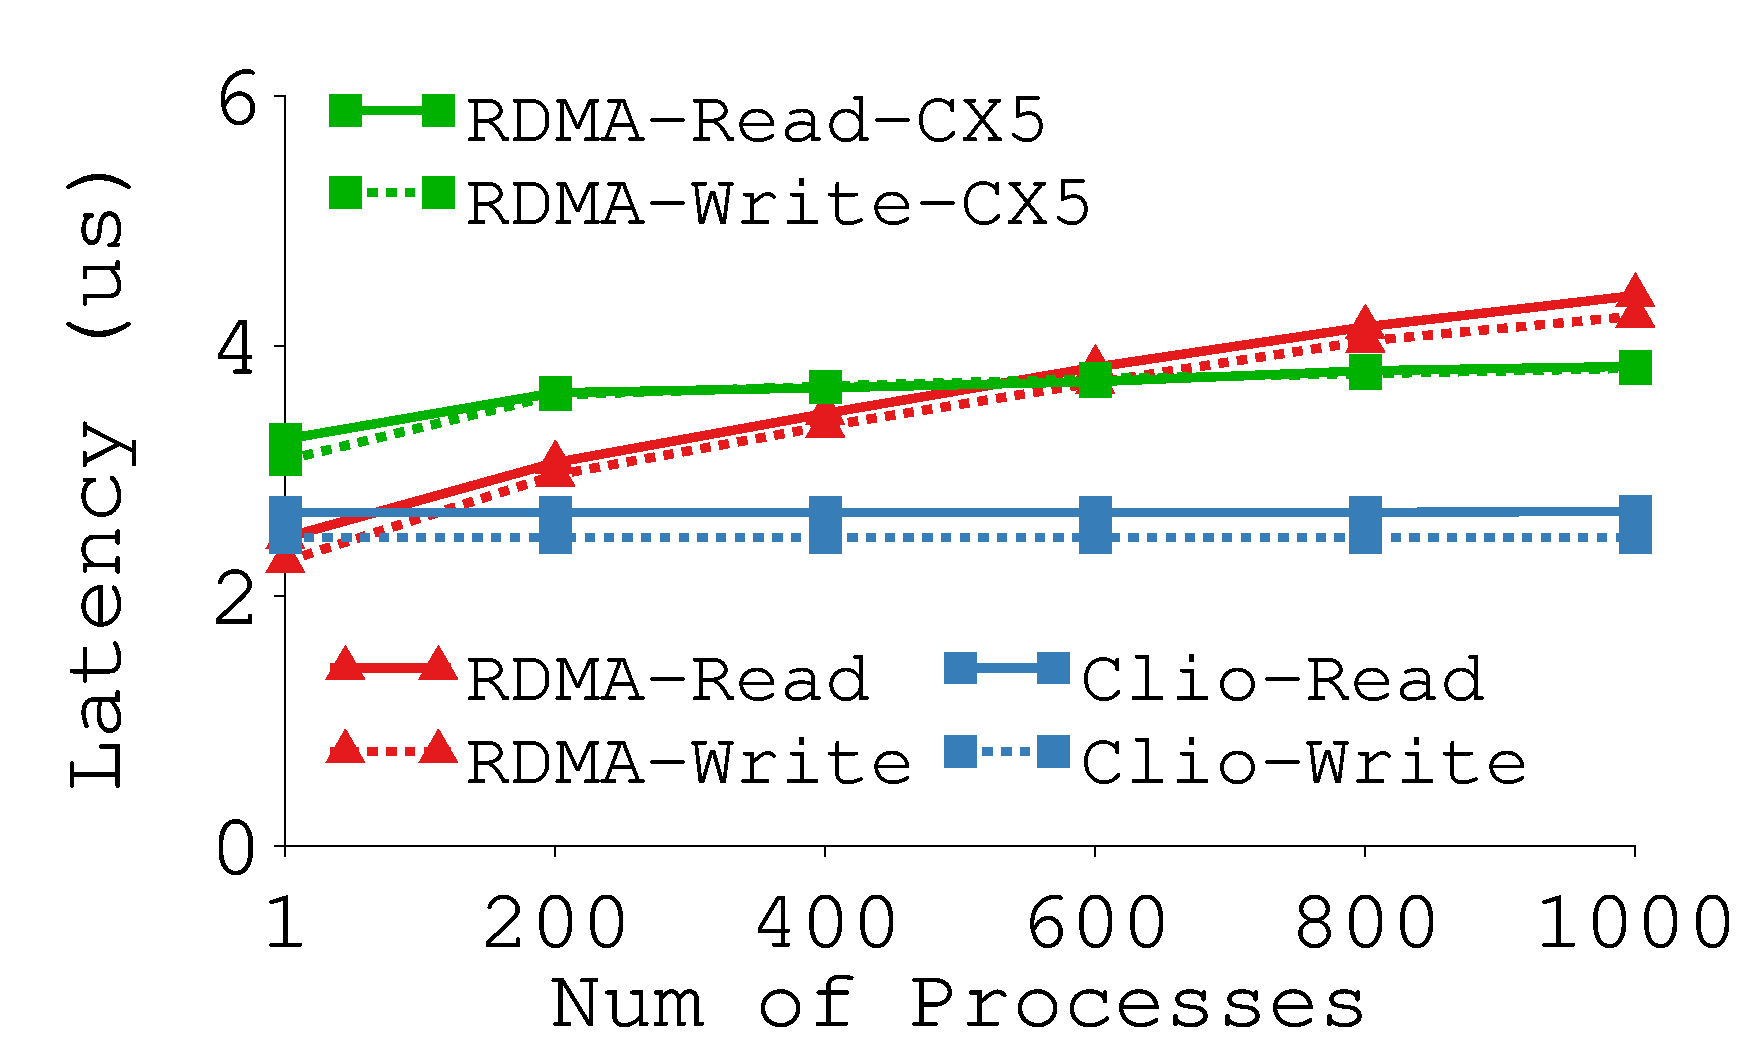
\includegraphics[width=\columnwidth]{Figures/g_plot_scalability_conn.pdf}}
\vspace{-0.1in}
\captionsetup{width=.9\columnwidth}
\mycaption{fig-conn}{Process (Connection) Scalability.}
{
}
\end{center}
\end{minipage}
%\begin{minipage}{0.01in}
%\hspace{0.01in}
%\end{minipage}
\begin{minipage}{\figWidthSix}
\begin{center}
\centerline{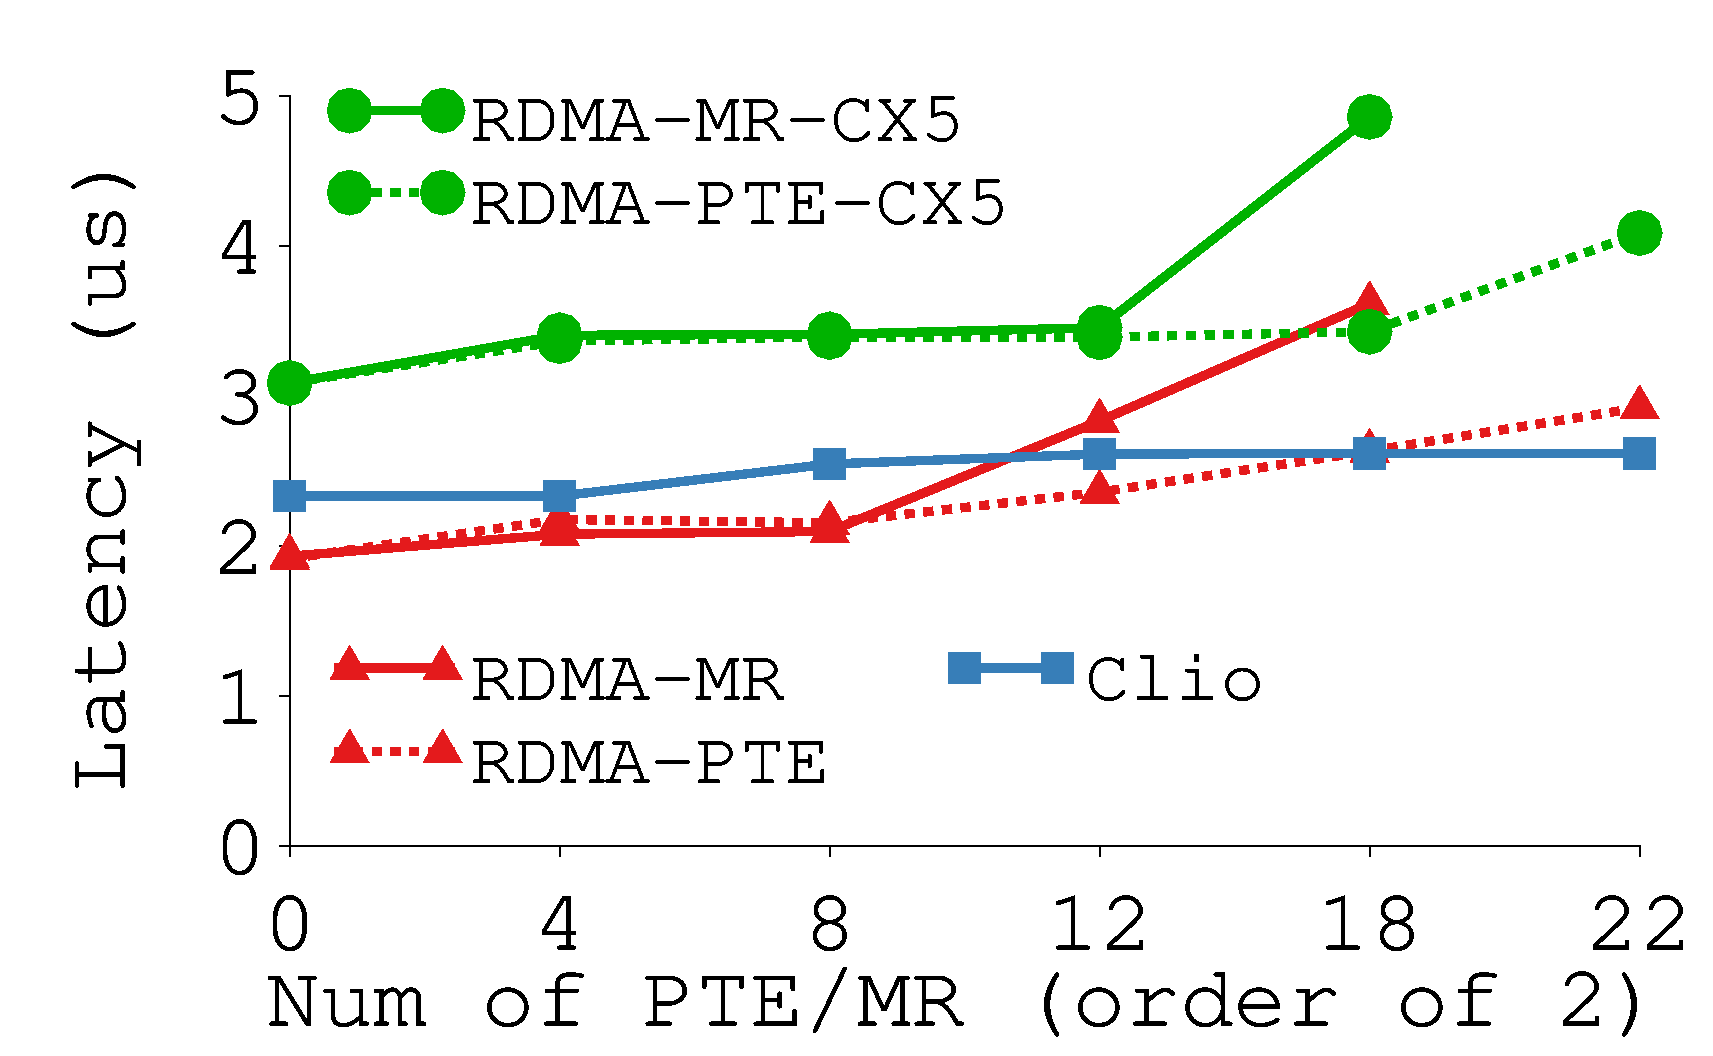
\includegraphics[width=\columnwidth]{Figures/g_plot_scalability_pte.pdf}}
\vspace{-0.1in}
\captionsetup{width=.9\columnwidth}
\mycaption{fig-pte-mr}{PTE and MR Scalability.}
{
RDMA fails beyond $2^{18}$ MRs. 
}
\end{center}
\end{minipage}
%\begin{minipage}{0.01in}
%\hspace{0.01in}
%\end{minipage}
\begin{minipage}{\figWidthSix}
\begin{center}
\centerline{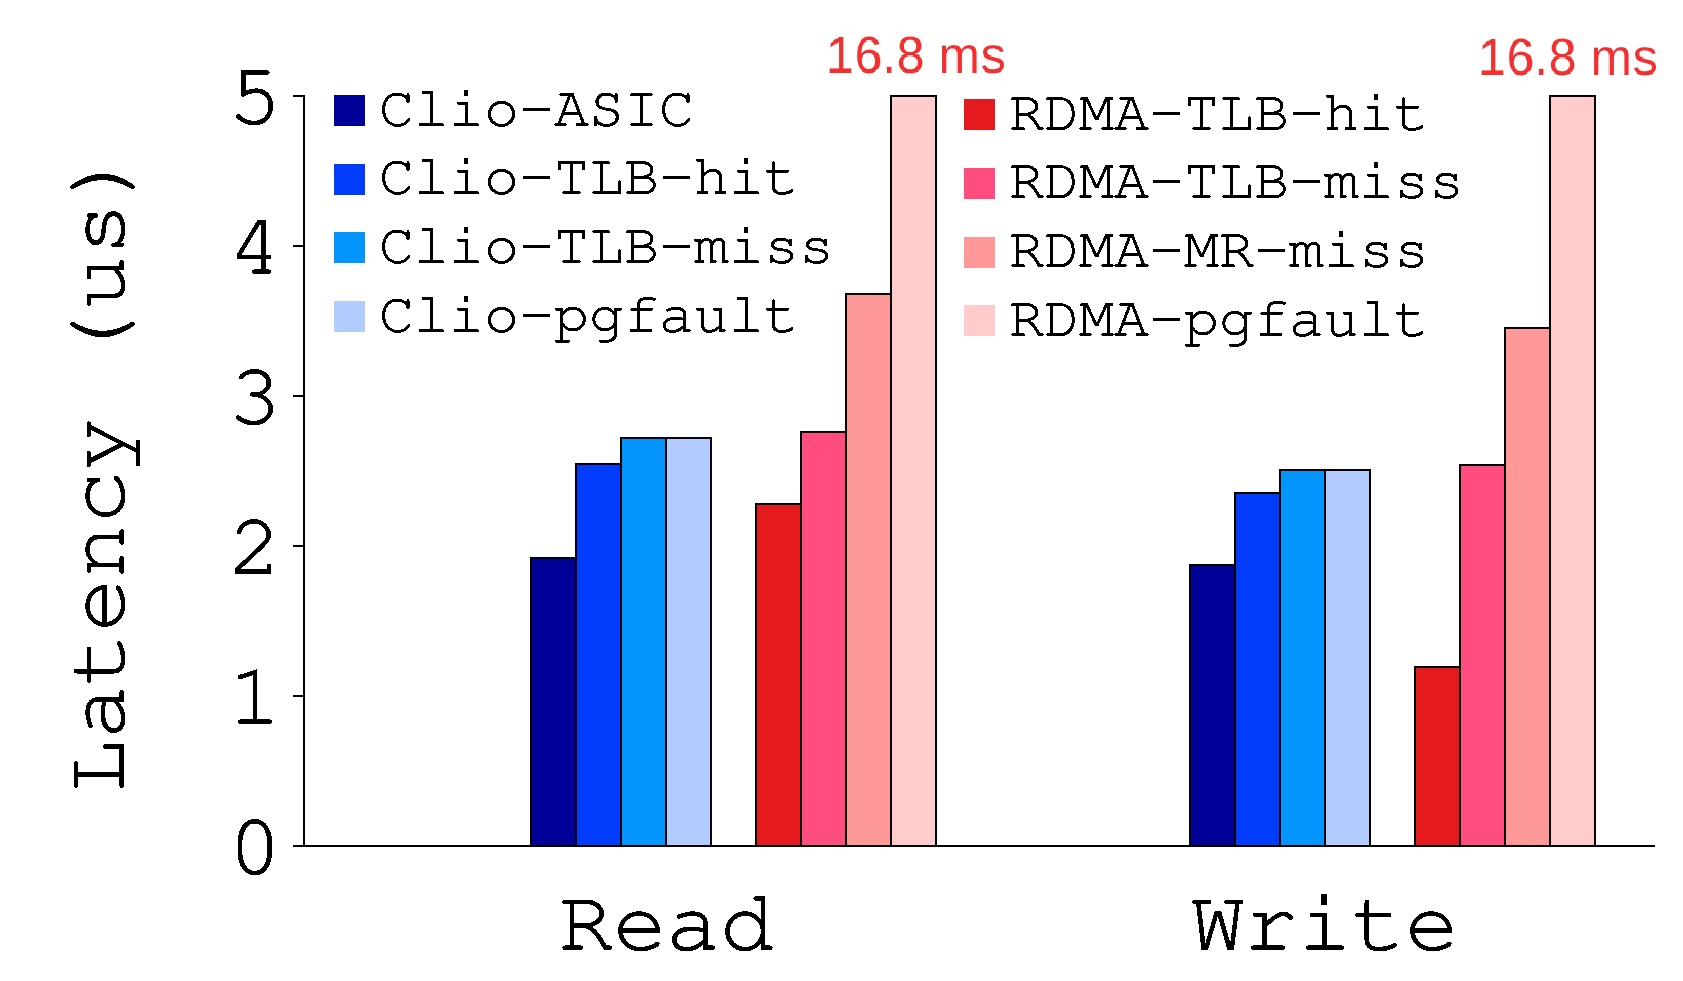
\includegraphics[width=\columnwidth]{Figures/g_plot_latency_comparison.pdf}}
\vspace{-0.1in}
\captionsetup{width=.9\columnwidth}
\mycaption{fig-miss-hit}{Comparison of TLB Miss and page fault.}
{
\sys-ASIC are projected values of TLB hit.
}
\end{center}
\end{minipage}
\begin{minipage}{\figWidthSix}
\begin{center}
\centerline{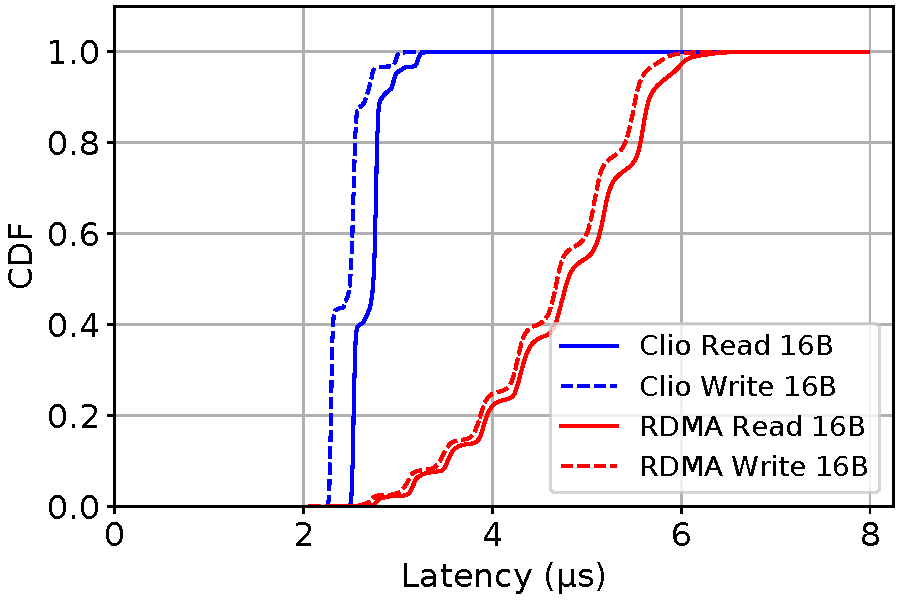
\includegraphics[width=\columnwidth]{Figures/clio_rdma_lat_cdf.pdf}}
\vspace{-0.1in}
\captionsetup{width=.9\columnwidth}
\mycaption{fig-tail-latency}{Latency CDF.}
{
}
\end{center}
\end{minipage}
\vspace{-0.1in}
\end{figure*}
}

{
\begin{figure*}[th]
\begin{center}
\centerline{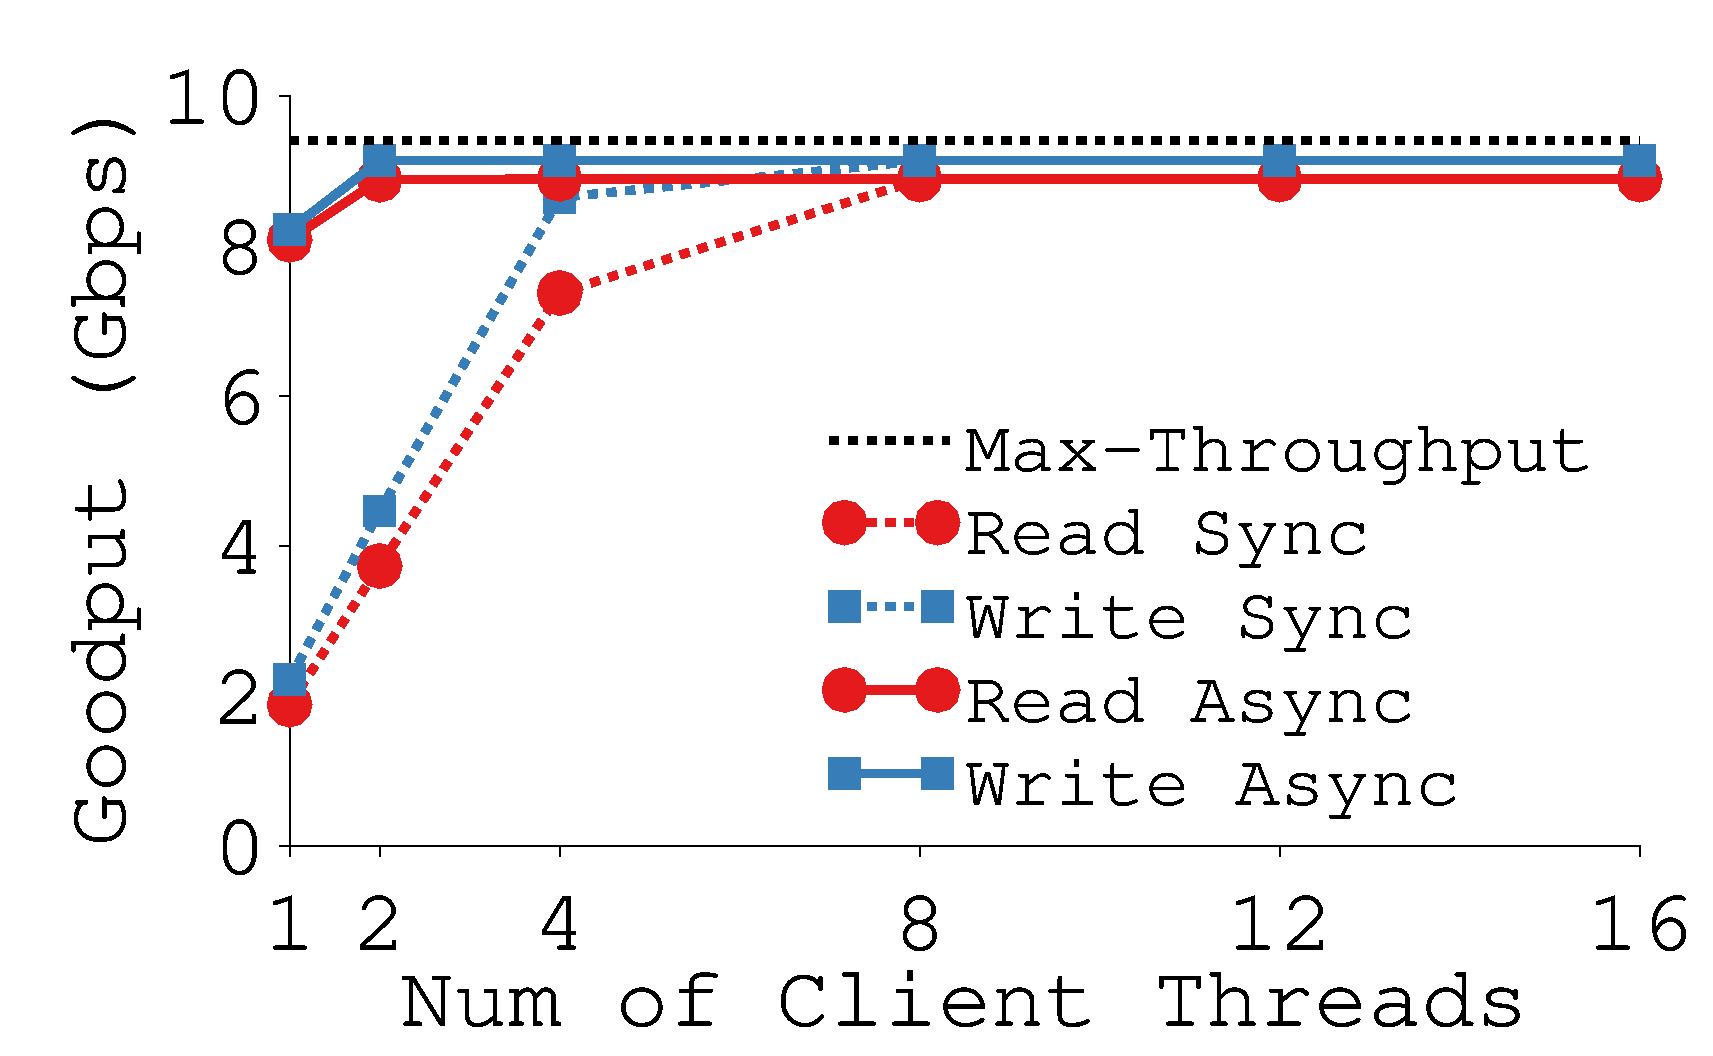
\includegraphics[width=0.5\textwidth]{clio/Figures/g_plot_throughput.pdf}}
\mycaption{fig-read-write-throughput}{End-to-End Goodput.}
{
1\KB\ requests. % between 1 \CN\ and 1 \MN.
}
\end{center}
\end{figure*}
}
{
\begin{figure*}[h]
\begin{center}
\centerline{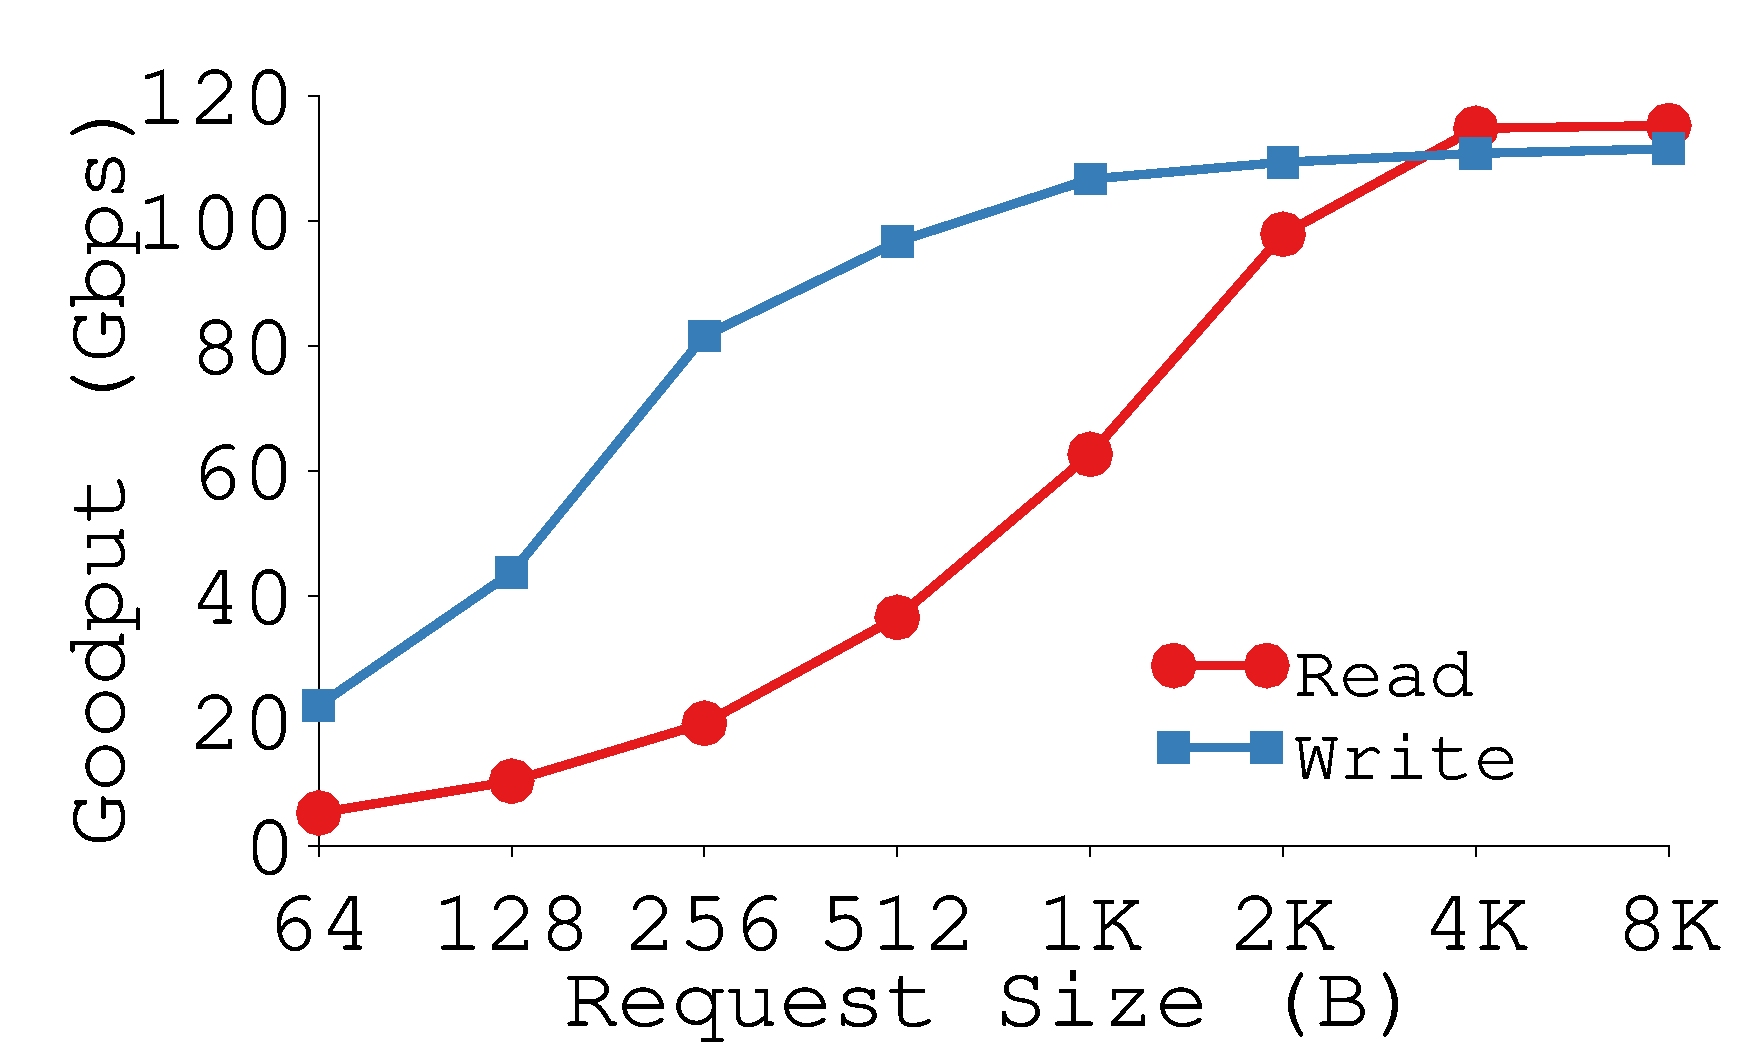
\includegraphics[width=0.5\textwidth]{clio/Figures/g_plot_onboard_throughput.pdf}}
\mycaption{fig-onboard-throughput}{On-board Goodput.}
{
FPGA test module generates requests at maximum speed.
}
\end{center}
\end{figure*}
}
{
\begin{figure*}[h]
\begin{center}
\centerline{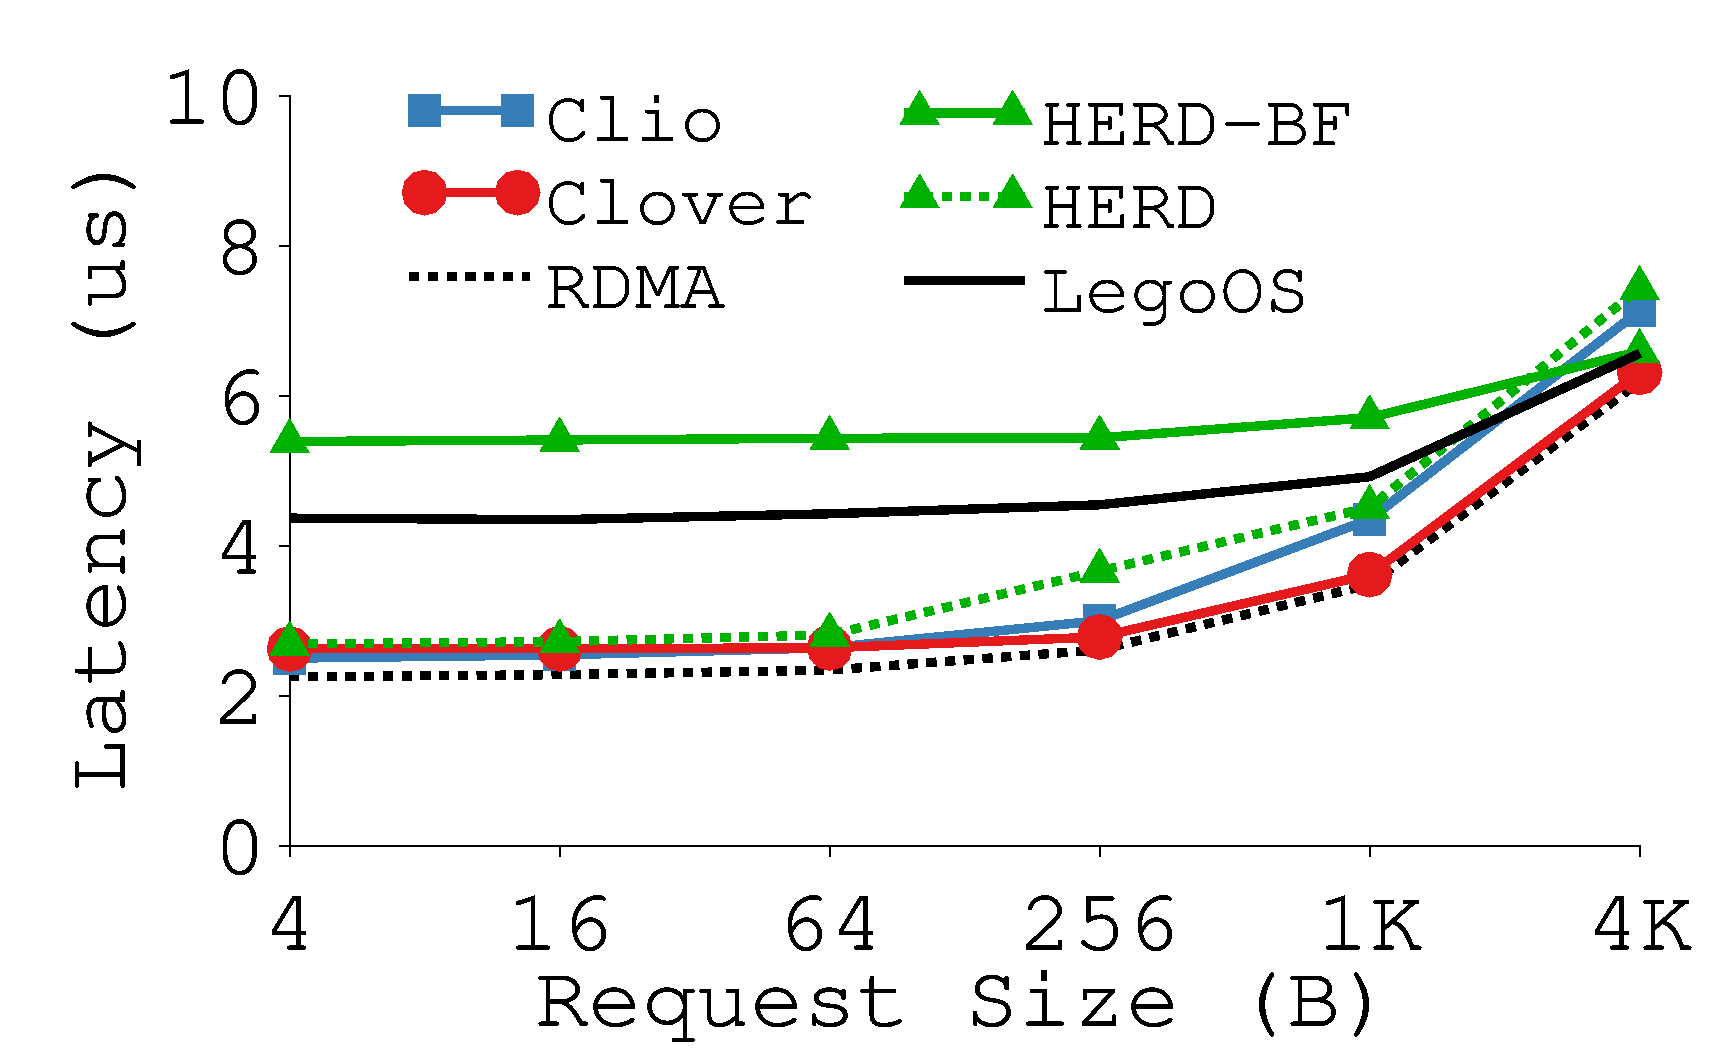
\includegraphics[width=0.5\textwidth]{clio/Figures/g_plot_read_latency.pdf}}
\mycaption{fig-read-lat}{Read Latency.}
{
HERD-BF: HERD running on BlueField. %SmartNIC.
}
\end{center}
\end{figure*}
}
{
\begin{figure*}[h]
\begin{center}
\centerline{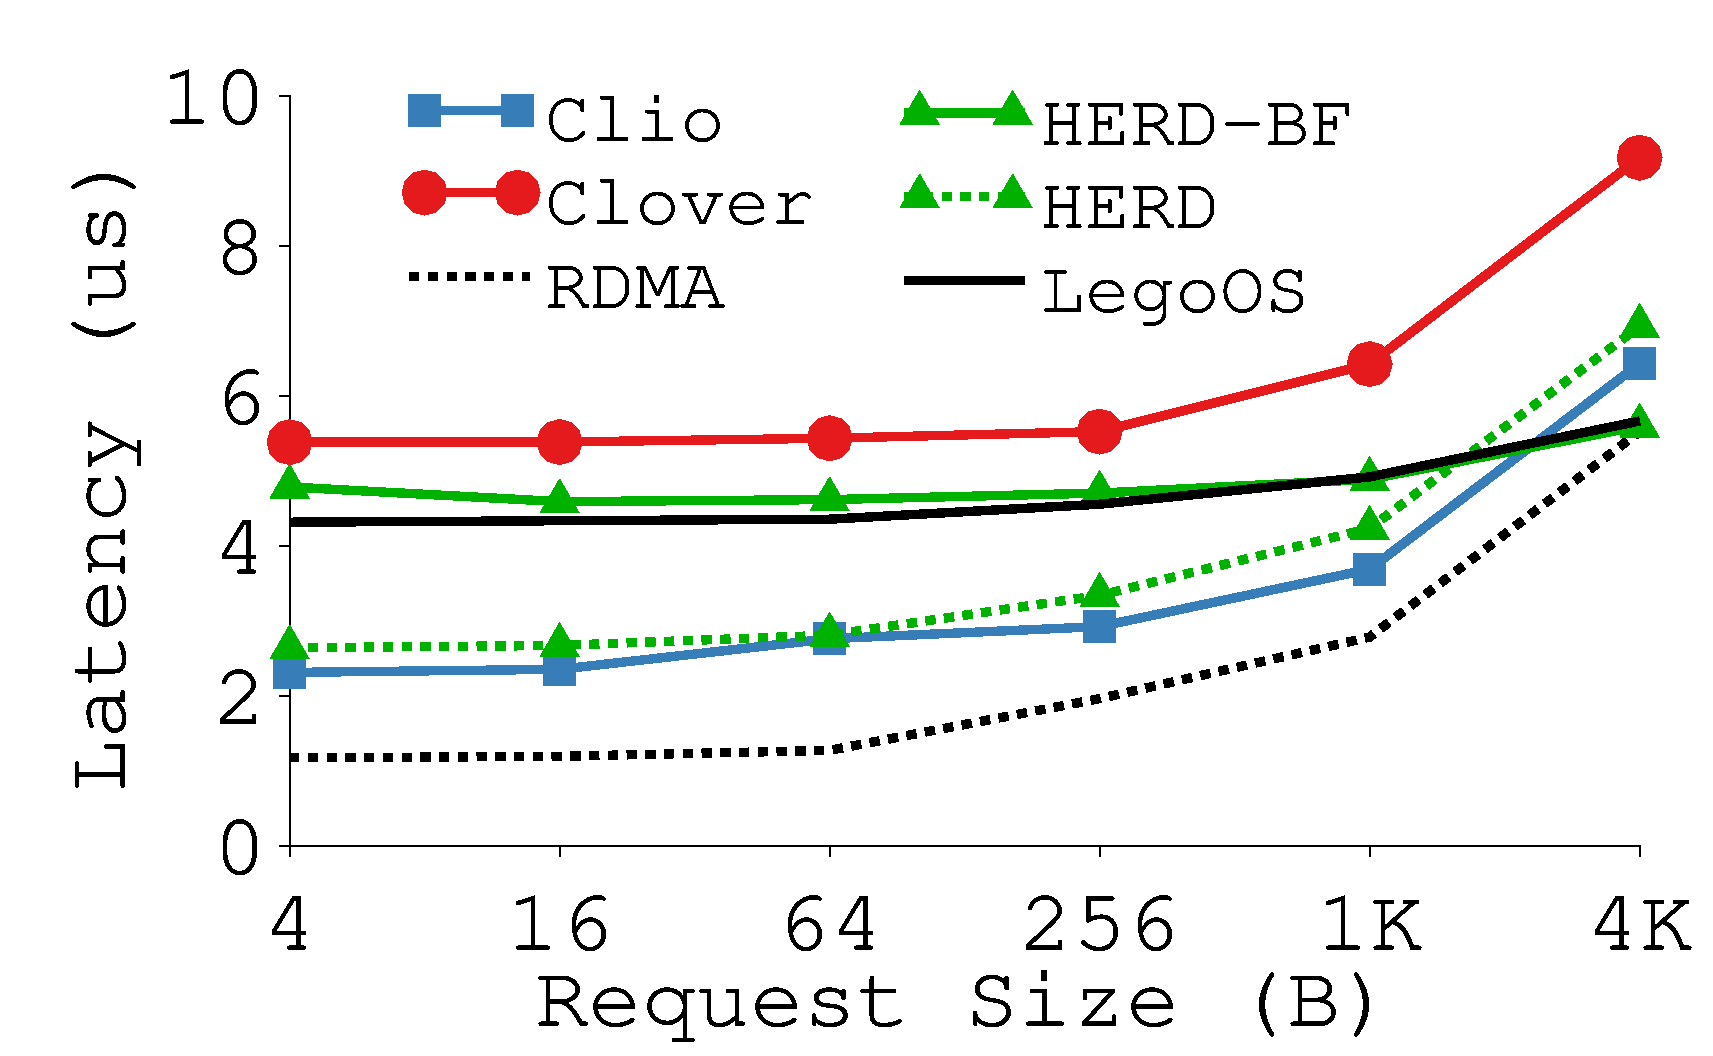
\includegraphics[width=0.5\textwidth]{clio/Figures/g_plot_write_latency.pdf}}
\mycaption{fig-write-lat}{Write Latency.}
{
Clover requires $\ge$ 2 RTTs for write.
}
\end{center}
\end{figure*}
}


\ulinebfpara{Key-value store.}
We built {\em \syskv}, a key-value store that supports concurrent 
create/update/read/delete key-value entries
with atomic write and read committed consistency.
\syskv\ runs at an \MN\ as a computation offloading module.
Users can access it through a key-value interface from multiple \CN{}s.
The \syskv\ module has its own virtual memory address space and uses \sys\ virtual memory APIs to access it.
\syskv\ uses a chained hash table in its virtual memory space for managing the metadata of key-value pairs, and it stores the actual key values at separate locations in the space.
Each hash bucket has a chain of slots. Each slot
contains the virtual addresses of seven key-value pairs.
It also stores a fingerprint for each key-value pair.

To create a new key-value pair, \syskv\ allocates space for
the key-value data with an \alloc\ call and writes the
data with an \Cliosyswrite. It then calculates the hash and the fingerprint of the key. 
Afterward, it fetches the last hash slot in the corresponding hash bucket using the hash value. If that
slot is full, \syskv\ allocates another slot using \alloc; otherwise, it just uses the fetched last slot. 
It then inserts the virtual address and fingerprint of the data into the last/new slot.
Finally, it links the current last slot to the new slot if a new one is created.

To perform a read, \syskv\ locates the hash bucket (with the key's hash value) and fetches one slot in the bucket
chain at a time using \Cliosysread. It then compares the fingerprint of the key to the seven entries in the slot. If there is no match, it
fetches the next slot in the bucket. Otherwise, with a matched
entry, it reads the key-value pair using the address stored in that
entry with an \Cliosysread. It then compares the full key and returns
the value if it is a match. Otherwise, it keeps searching the bucket.

The above describes a single-\MN\ \syskv\ system. Another \CN-side load balancer is used to partition key-value pairs into different \MN{}s.
Since all \CN{}s requests of the same partition go to the same \MN\ and \sys\ APIs within an \MN\ are properly ordered, it is fairly easy for \syskv\ to guarantee the atomic-write, read-committed consistency level.

We implemented \syskv\ with 772 SpinalHDL code in 6 developer days.
To evaluate \sys's virtual memory API overhead at \sysboard, we also implemented a key-value store with the same design as \syskv\ but with raw physical memory interface.
This physical-memory-based implementation takes more time to develop and only yields 4\%–12\% latency improvement and 1\%–5\% throughput improvement over \syskv. %\yiying{Zhiyuan, do you still remember or can estimate how much longer does the physical memory one take than our final virtual memory one?}
%\zhiyuan{basically we only replace the DMA module with physical DMA and legomem-VA DMA. So the effort should remains the same. The extra work for PA is handling the memory management, but that part is very simple for the current impl. I'll get details later}
%\zhiyuan{Also easy change from physical DMA to virtual DMA can be seens as easy adoption to Clio? 27 lines added on top of phys compared to 809 lines of code}
%\yiying{What is 809 LOC? 809 for the original phys impl? and to change it to virt, we replace 809 lines with 27 lines?} \zhiyuan{we add 27 line on top of 908 to adopt the original phys code to use Clio virtual memory}



\ulinebfpara{Multi-version object store.}
We built a multi-version object store ({\em \sysmv}) which lets users on \CN{}s create an object, append a new version to an object, 
read a specific version  or the latest version of an object, and delete an object.
Similar to \syskv, \sysmv\ has its own address space.
In the address space, it uses an array to store versions of data for each object, a map to store the mapping from object IDs to the per-object array addresses, and a list to store free object IDs. 
When a new object is created, \sysmv\ allocates a new array (with \alloc) 
and writes the virtual memory address of the array into the object ID map.
Appending a new version to an object simply increases the latest version number
and uses that as an index to the object array for writing the value.
Reading a version simply reads the corresponding element of the array.

\sysmv\ allows concurrent accesses from \CN{}s to an object and guarantees sequential consistency for each object.
Each \sysmv\ user request involves at least two internal
\sys\ operations, some of which include both metadata and
data operations. This compound request pattern makes it tricky
to deal with synchronization problems, as \sysmv\ needs to
ensure that no internal \sys\ operation of a later \sysmv\ request could affect the correctness of an earlier \sysmv\ request. 
% Fortunately, both \sys's fast path and slow path guarantee sequential delivery of \sys\ operations. Since \sysmv\ only issues one Clio operation per
% clock cycle, the ordering that \sys\ modules guarantee is sufficient to deliver \sysmv’s consistency guarantees. 
We implemented \sysmv\ with 1680 lines of C HLS code in 15 developer days.
 
\ulinebfpara{Simple data analytics.}
Our final example is a simple DataFrame-like data processing application ({\em \sysdf}),
which splits its computation between \CN\ and \MN.
We implement \texttt{select} and \texttt{aggregate} at \MN\ as two offloads,
as offloading them can reduce the amount of data sent over the network.
We keep other operations like \texttt{shuffle} and \texttt{histogram} at \CN.
For the same user, all these modules share the same address space regardless of whether they are at \CN\ or \MN.
Thanks to \sys's support of computation offloading sharing the same address space as computations running at host, \sysdf's implementation is largely simplified and its performance is improved by avoiding data serialization/deserialization.
We implemented \sysdf\ with 202 lines of SpinalHDL code and 170 lines of C interface code in 7 developer days.

